\section{Preventivo}
In questa sezione del documento si può trovare come sono state distribuite le risorse del gruppo nelle varie fasi di lavoro.\\
Inoltre sono illustrate la pianificazione e distribuzione oraria dei ruoli per ogni membro del gruppo, i quali devono:
\begin{itemize}
	\item ricoprire tutti i ruoli durante tutta la durata del progetto;
	\item avere circa le stesse ore produttive alla fine di ogni fase del progetto;
\end{itemize}
Inoltre il verificatore di un determinato task non potrà essere colui che lo ha svolto.\\
Il riferimento alle sigle identificative dei ruoli si può trovare al paragrafo 3.1.3.5 del documento Norme di Progetto.

\subsection{Analisi dei requisiti}
%
% ----------------------------------------------------------------------------------------------------------------
\subsubsection{Periodo 1}
% ----------------------------------------------------------------------------------------------------------------
%
\subsubsubsection{Preventivo ore}
\begin{table}[h]
	\setlength\extrarowheight{5pt}
	\centering
	\rowcolors{2}{gray!10}{gray!40}
	\begin{tabularx}{\textwidth}{|ccccccc|c|}
		\hline
		\rowcolor{white}
		\textbf{Nome} & \textbf{Re} & \textbf{Am} & \textbf{An} & \textbf{Ve} & \textbf{Pr}& \textbf{Pt} & \textbf{Ore totali} \\
		\hline
		Nicola Sinicato &3&3&4&0&0&0&10 \\
		Gabriele Da Re &0&6&4&0&0&0&10 \\
		Luca Brugnera &0&6&4&0&0&0&10 \\
		Matteo Stocco &1&5&4&0&0&0&10 \\
		Ana Lazic &1&3&6&0&0&0&10 \\
		Zhen Wei Zheng &1&3&6&0&0&0&10 \\
		\hline
		Ore totali ruolo &6&26&28&0&0&0&60 \\
		\hline
	\end{tabularx}
	\vspace{10pt}
	\caption{Tabella 10: Distribuzione ore durante la fase di analisi per ruolo e persona}
\end{table}
\subsubsubsection{Preventivo costi}
\begin{table}[h]
	\setlength\extrarowheight{5pt}
	\centering
	\rowcolors{2}{gray!10}{gray!40}
	\begin{tabularx}{\textwidth}{|ccc|c|}
		\hline
		\rowcolor{white}
		\textbf{Ruolo} & \textbf{Costo orario (€)} & \textbf{Ore totali} & \textbf{Costo totale (€)} \\
		\hline
		Responsabile &30&6&180 \\
		Amministratore &20&26&520 \\
		Analista &25&28&700 \\
		Verificatore &15&0&0 \\
		Programmatore &15&0&0 \\
		Progettista &25&0&0 \\
		\hline
		Totale &-&-&1400 \\
		\hline
	\end{tabularx}
    \vspace{10pt}
	\caption{Tabella 11: Distribuzione ore durante la fase di analisi per ruolo}
\end{table}
\begin{figure}[H]
    \centering
    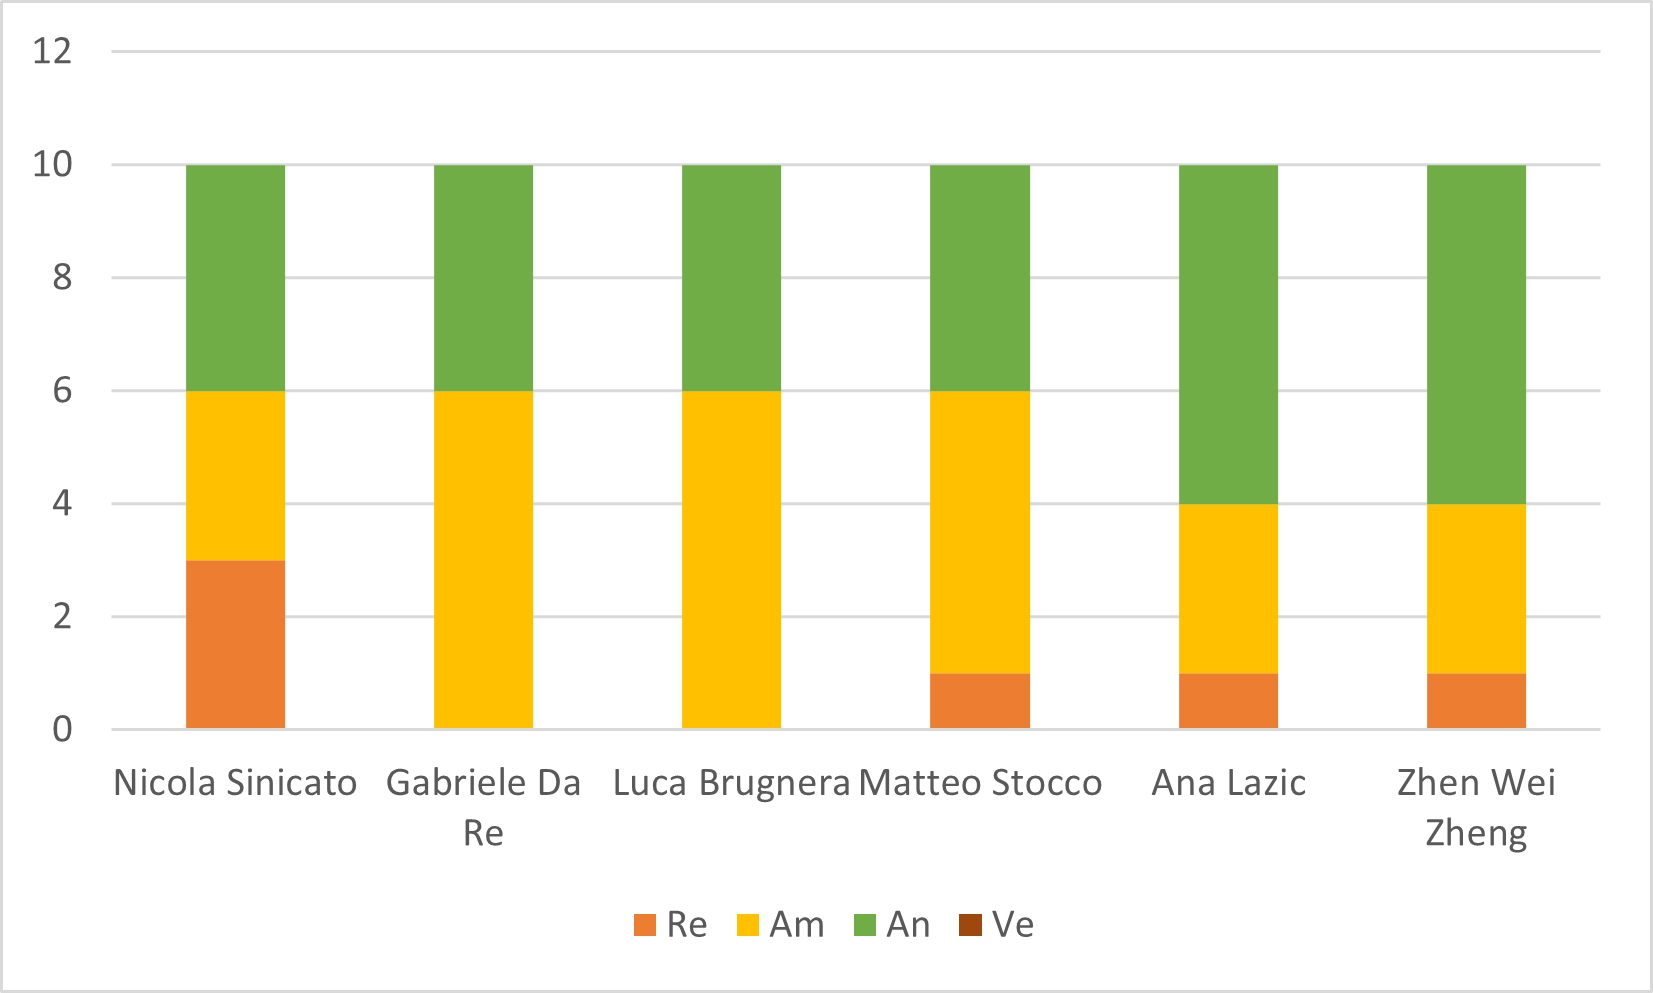
\includegraphics[scale=0.6]{img/grafi preventivo/istogrammi/analisi/periodo1.png}
    \caption{Istogramma per la distribuzione oraria durante la fase di analisi}
\end{figure}
\begin{figure}[H]
    \centering
    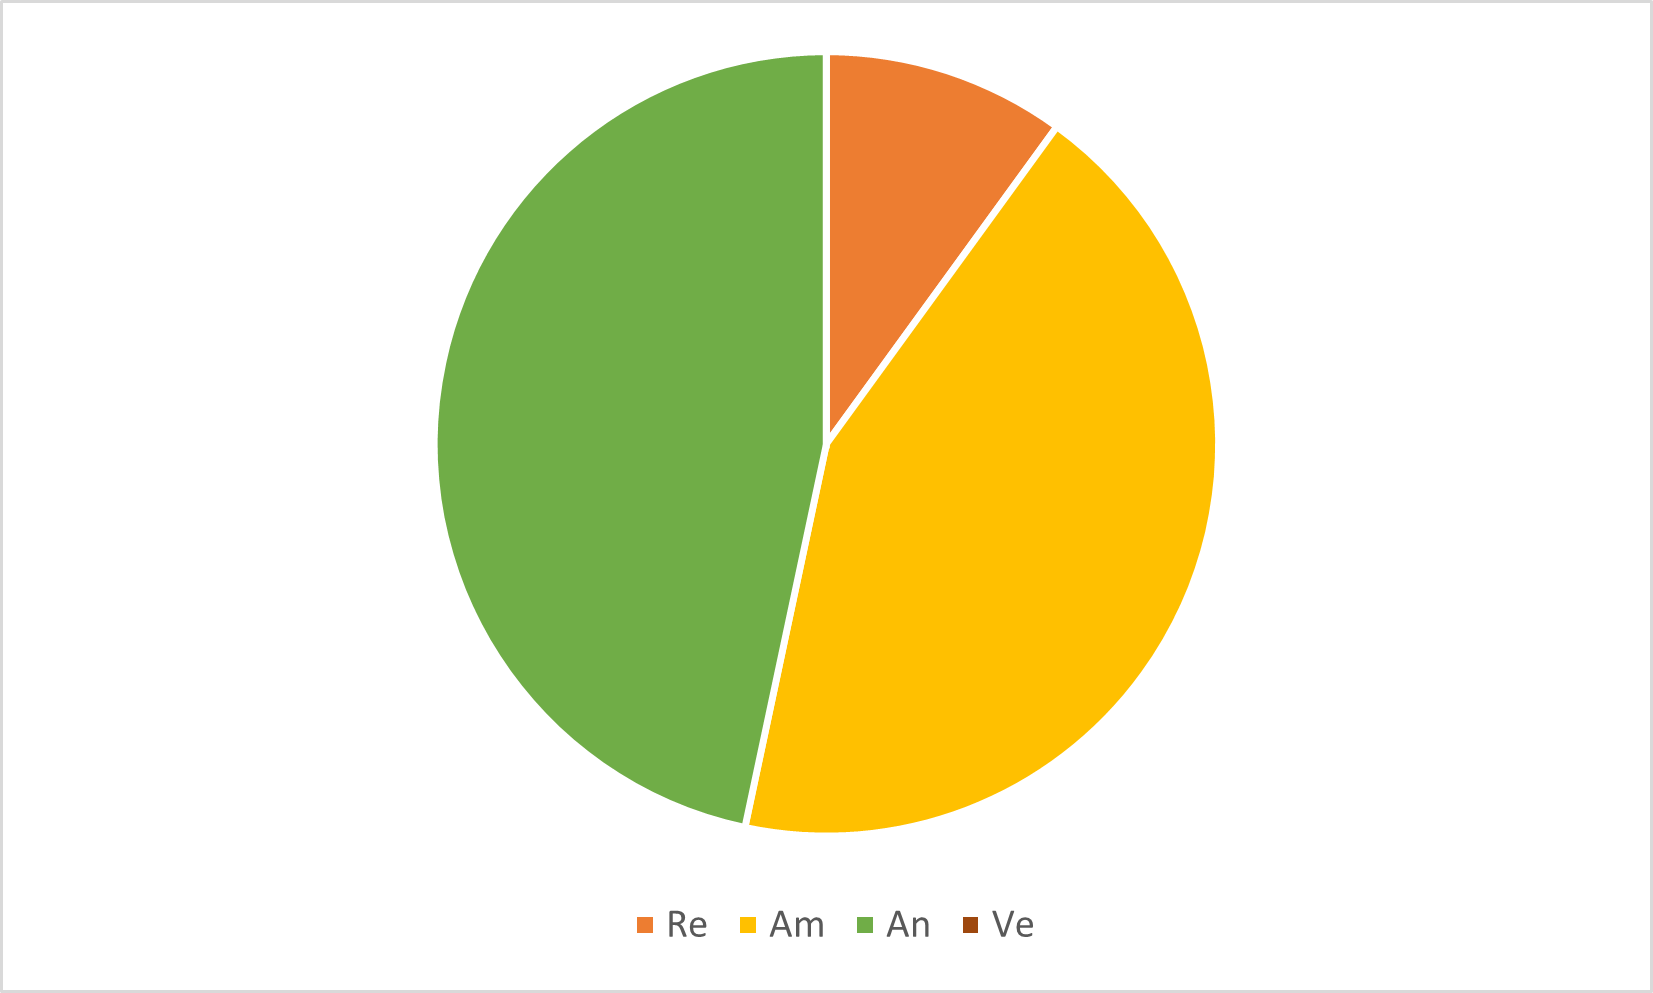
\includegraphics[scale=0.6]{img/grafi preventivo/torta/analisi/periodo1.png}
    \caption{Rappresentazione delle ore impiegate per ruolo durante la fase di analisi}
\end{figure}
%
% ----------------------------------------------------------------------------------------------------------------
\subsubsection{Periodo 2}
% ----------------------------------------------------------------------------------------------------------------
%
\subsubsubsection{Preventivo ore}
\begin{table}[h]
	\setlength\extrarowheight{5pt}
	\centering
	\rowcolors{2}{gray!10}{gray!40}
	\begin{tabularx}{\textwidth}{|ccccccc|c|}
		\hline
		\rowcolor{white}
		\textbf{Nome} & \textbf{Re} & \textbf{Am} & \textbf{An} & \textbf{Ve} & \textbf{Pr}& \textbf{Pt} & \textbf{Ore totali} \\
		\hline
		Nicola Sinicato &2&1&8&4&0&0&15 \\
		Gabriele Da Re &1&4&7&3&0&0&15 \\
		Luca Brugnera &1&5&6&3&0&0&15 \\
		Matteo Stocco &2&2&7&4&0&0&15 \\
		Ana Lazic &0&2&7&4&0&0&15 \\
		Zhen Wei Zheng &0&2&6&7&0&0&15 \\
		\hline
		Ore totali ruolo &6&16&41&27&0&0&90 \\
		\hline
	\end{tabularx}
	\vspace{10pt}
	\caption{Tabella 10: Distribuzione ore durante la fase di analisi per ruolo e persona}
\end{table}
\subsubsubsection{Preventivo costi}
\begin{table}[h]
	\setlength\extrarowheight{5pt}
	\centering
	\rowcolors{2}{gray!10}{gray!40}
	\begin{tabularx}{\textwidth}{|ccc|c|}
		\hline
		\rowcolor{white}
		\textbf{Ruolo} & \textbf{Costo orario (€)} & \textbf{Ore totali} & \textbf{Costo totale (€)} \\
		\hline
		Responsabile &30&6&180 \\
		Amministratore &20&16&320 \\
		Analista &25&41&1025 \\
		Verificatore &15&27&405 \\
		Programmatore &15&0&0 \\
		Progettista &25&0&0 \\
		\hline
		Totale &-&-&1930 \\
		\hline
	\end{tabularx}
    \vspace{10pt}
	\caption{Tabella 11: Distribuzione ore durante la fase di analisi per ruolo}
\end{table}
\begin{figure}[H]
    \centering
    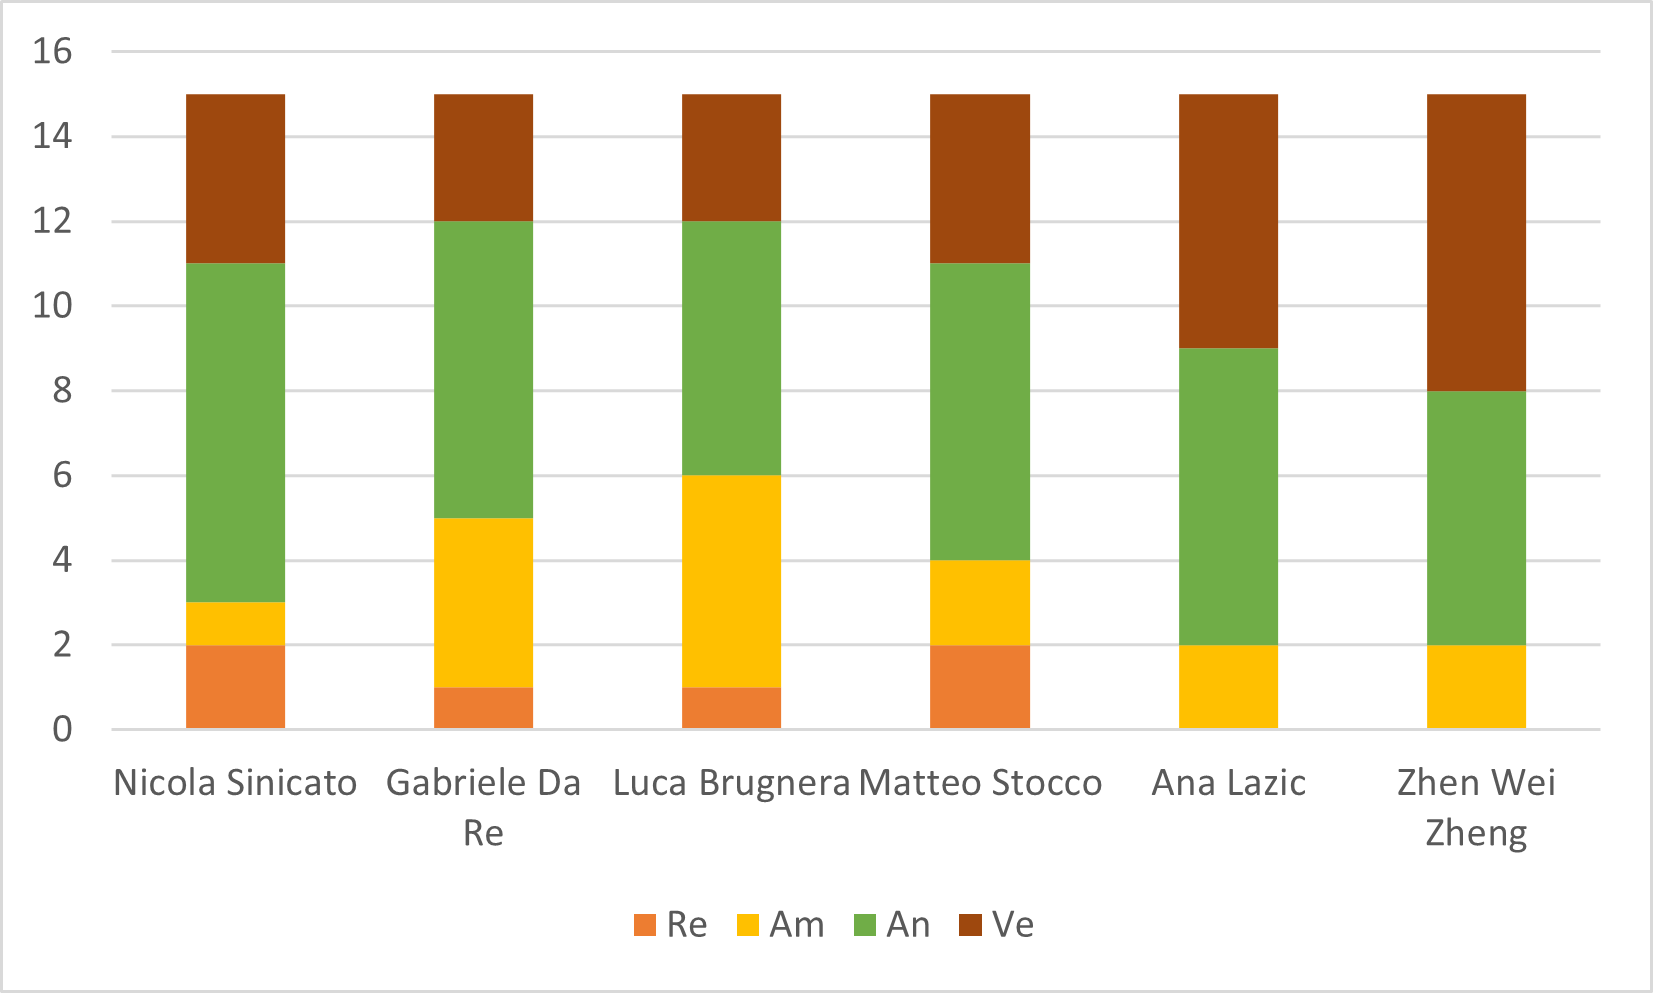
\includegraphics[scale=0.6]{img/grafi preventivo/istogrammi/analisi/periodo2.png}
    \caption{Istogramma per la distribuzione oraria durante la fase di analisi}
\end{figure}
\begin{figure}[H]
    \centering
    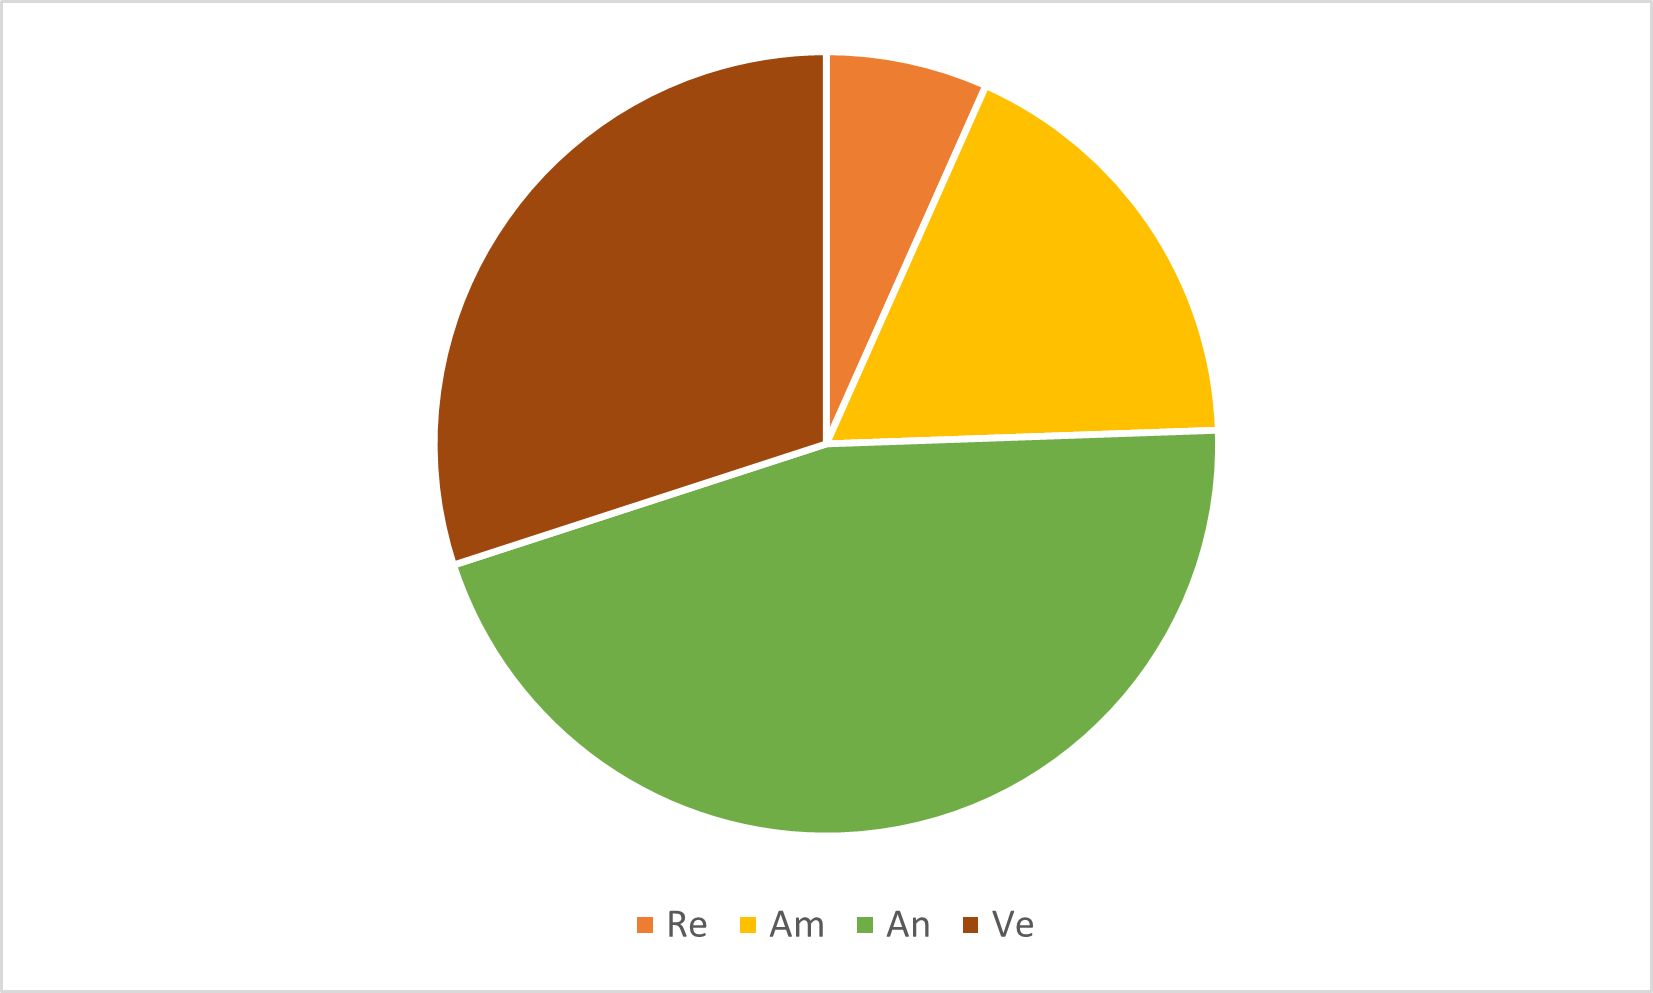
\includegraphics[scale=0.6]{img/grafi preventivo/torta/analisi/periodo2.png}
    \caption{Rappresentazione delle ore impiegate per ruolo durante la fase di analisi}
\end{figure}
%
% ----------------------------------------------------------------------------------------------------------------
\subsubsection{Periodo 3}
% ----------------------------------------------------------------------------------------------------------------
%
\subsubsubsection{Preventivo ore}
\begin{table}[h]
	\setlength\extrarowheight{5pt}
	\centering
	\rowcolors{2}{gray!10}{gray!40}
	\begin{tabularx}{\textwidth}{|ccccccc|c|}
		\hline
		\rowcolor{white}
		\textbf{Nome} & \textbf{Re} & \textbf{Am} & \textbf{An} & \textbf{Ve} & \textbf{Pr}& \textbf{Pt} & \textbf{Ore totali} \\
		\hline
		Nicola Sinicato &0&1&2&2&0&0&5 \\
		Gabriele Da Re &1&2&1&1&0&0&5 \\
		Luca Brugnera &0&2&1&2&0&0&5 \\
		Matteo Stocco &1&0&2&2&0&0&5 \\
		Ana Lazic &1&0&3&1&0&0&5 \\
		Zhen Wei Zheng &0&0&2&3&0&0&5 \\
		\hline
		Ore totali ruolo &3&5&11&11&0&0&30 \\
		\hline
	\end{tabularx}
	\vspace{10pt}
	\caption{Tabella 10: Distribuzione ore durante la fase di analisi per ruolo e persona}
\end{table}
\subsubsubsection{Preventivo costi}
\begin{table}[h]
	\setlength\extrarowheight{5pt}
	\centering
	\rowcolors{2}{gray!10}{gray!40}
	\begin{tabularx}{\textwidth}{|ccc|c|}
		\hline
		\rowcolor{white}
		\textbf{Ruolo} & \textbf{Costo orario (€)} & \textbf{Ore totali} & \textbf{Costo totale (€)} \\
		\hline
		Responsabile &30&3&90 \\
		Amministratore &20&5&100 \\
		Analista &25&11&00275 \\
		Verificatore &15&11&165 \\
		Programmatore &15&0&0 \\
		Progettista &25&0&0 \\
		\hline
		Totale &-&-&630 \\
		\hline
	\end{tabularx}
    \vspace{10pt}
	\caption{Tabella 11: Distribuzione ore durante la fase di analisi per ruolo}
\end{table}
\begin{figure}[H]
    \centering
    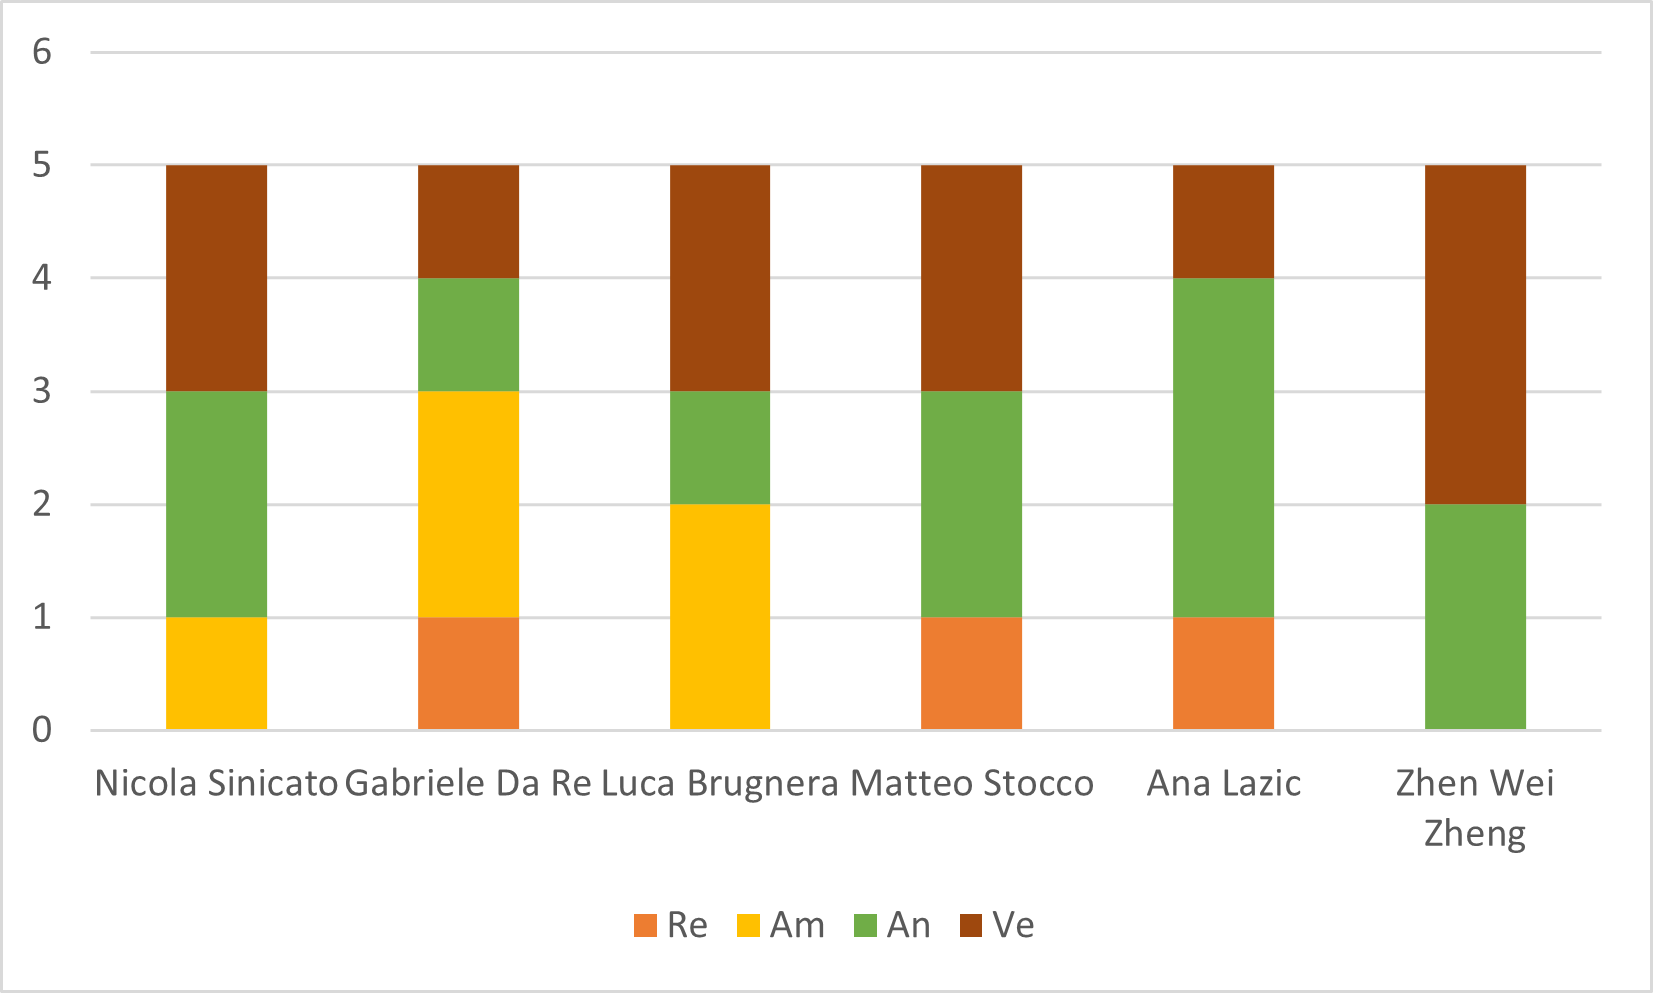
\includegraphics[scale=0.6]{img/grafi preventivo/istogrammi/analisi/periodo3.png}
    \caption{Istogramma per la distribuzione oraria durante la fase di analisi}
\end{figure}
\begin{figure}[H]
    \centering
    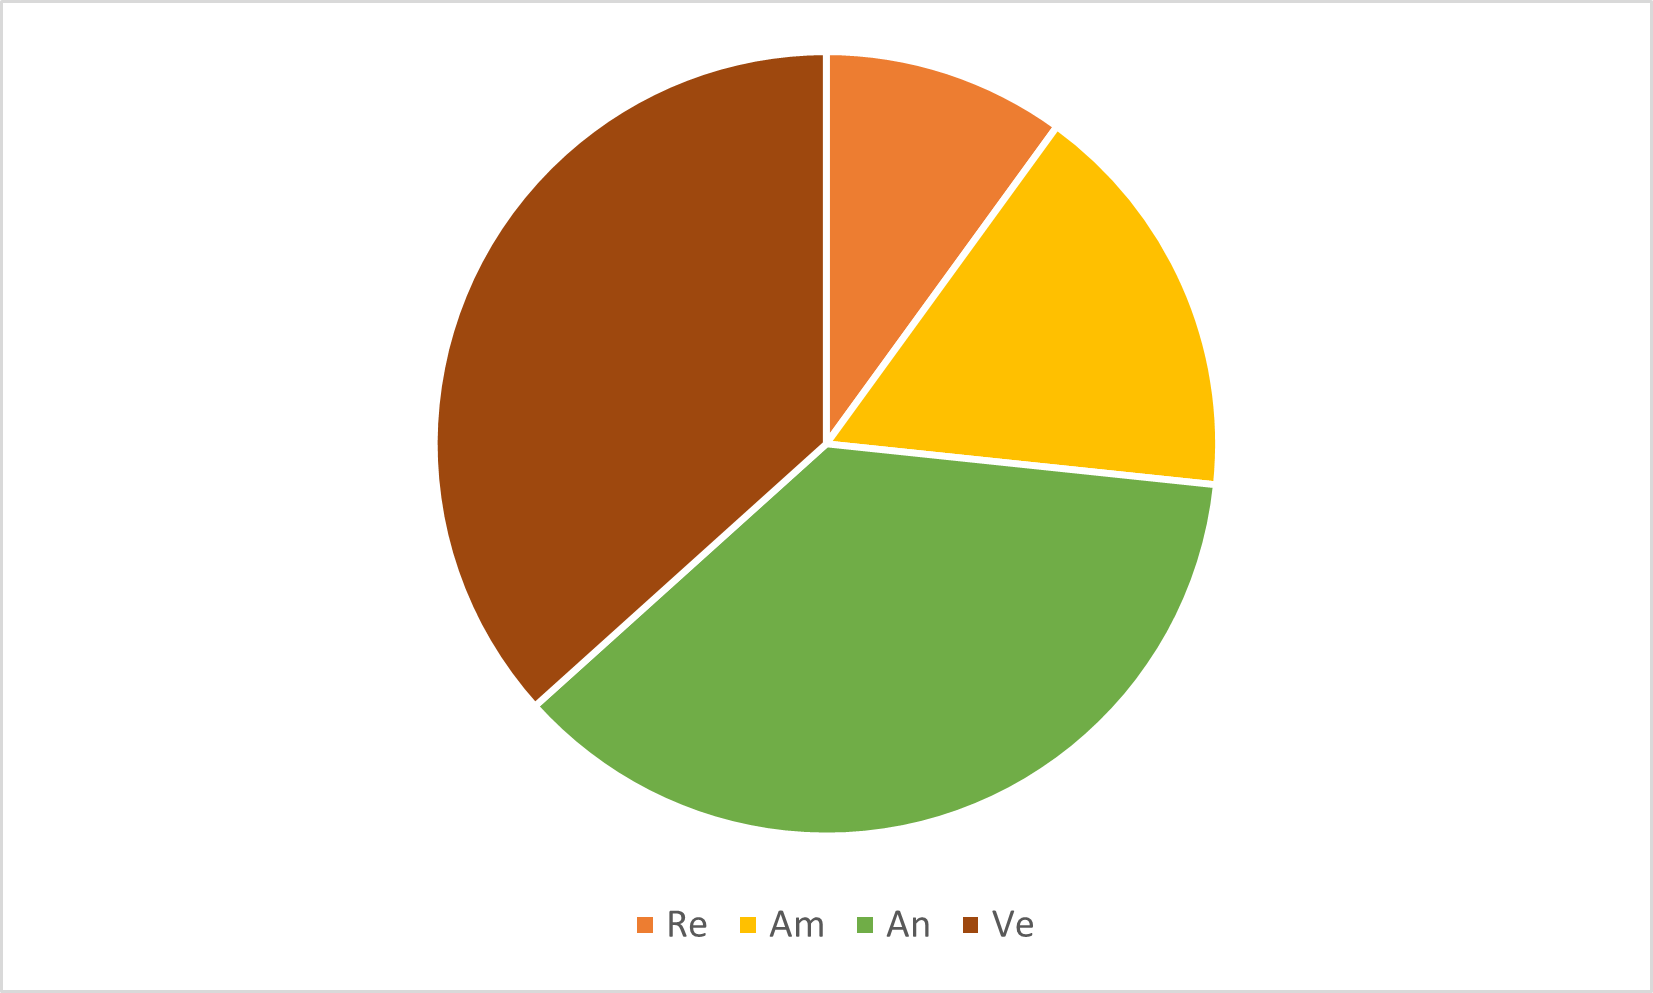
\includegraphics[scale=0.6]{img/grafi preventivo/torta/analisi/periodo3.png}
    \caption{Rappresentazione delle ore impiegate per ruolo durante la fase di analisi}
\end{figure}
%
% ----------------------------------------------------------------------------------------------------------------
\subsubsection{Complessivo periodo di analisi}
% ----------------------------------------------------------------------------------------------------------------
%
\subsubsubsection{Preventivo ore}
\begin{table}[h]
	\setlength\extrarowheight{5pt}
	\centering
	\rowcolors{2}{gray!10}{gray!40}
	\begin{tabularx}{\textwidth}{|ccccccc|c|}
		\hline
		\rowcolor{white}
		\textbf{Nome} & \textbf{Re} & \textbf{Am} & \textbf{An} & \textbf{Ve} & \textbf{Pr}& \textbf{Pt} & \textbf{Ore totali} \\
		\hline
		Nicola Sinicato &5&5&14&6&0&0&30 \\
		Gabriele Da Re &2&12&12&4&0&0&30 \\
		Luca Brugnera &1&13&11&5&0&0&30 \\
		Matteo Stocco &4&7&13&6&0&0&30 \\
		Ana Lazic &2&5&16&7&0&0&30 \\
		Zhen Wei Zheng &1&5&14&10&0&0&30 \\
		\hline
		Ore totali ruolo &15&47&80&38&0&0&180 \\
		\hline
	\end{tabularx}
	\vspace{10pt}
	\caption{Tabella 10: Distribuzione ore durante la fase di analisi per ruolo e persona}
\end{table}
\subsubsubsection{Preventivo costi}
\begin{table}[h]
	\setlength\extrarowheight{5pt}
	\centering
	\rowcolors{2}{gray!10}{gray!40}
	\begin{tabularx}{\textwidth}{|ccc|c|}
		\hline
		\rowcolor{white}
		\textbf{Ruolo} & \textbf{Costo orario (€)} & \textbf{Ore totali} & \textbf{Costo totale (€)} \\
		\hline
		Responsabile &30&15&450 \\
		Amministratore &20&47&940 \\
		Analista &25&80&2000 \\
		Verificatore &15&38&570 \\
		Programmatore &15&0&0 \\
		Progettista &25&0&0 \\
		\hline
		Totale &-&-&3960 \\
		\hline
	\end{tabularx}
    \vspace{10pt}
	\caption{Tabella 11: Distribuzione ore durante la fase di analisi per ruolo}
\end{table}
\begin{figure}[H]
    \centering
    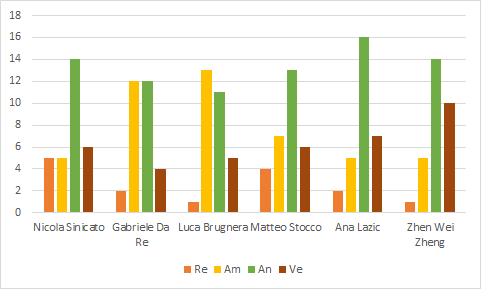
\includegraphics[scale=0.6]{img/grafi preventivo/istogrammi/analisi/totale.png}
    \caption{Istogramma per la distribuzione oraria durante la fase di analisi}
\end{figure}
\begin{figure}[H]
    \centering
    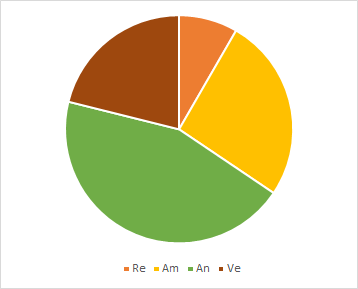
\includegraphics[scale=0.6]{img/grafi preventivo/torta/analisi/totale.png}
    \caption{Rappresentazione delle ore impiegate per ruolo durante la fase di analisi}
\end{figure}

